% Probability PageRank Markov Process
%
% File:         probability-pagerank-markov-process.tex
% Author:       Bob Walton (walton@acm.org)
% Date:      	Tue Jan  1 09:56:56 EST 2013
  
\documentclass{minimal}
\usepackage[paperheight=3.3in,paperwidth=5.0in,
            height=3.3in,hoffset=0.05in,
	    voffset=0.05in,left=0in,width=5.0in]{geometry}
\usepackage{ifthen}
\usepackage{color}
\usepackage[usenames]{xcolor}
\usepackage{scalefnt}
\usepackage{tikz}
\newcommand{\SMALL}{\scalefont{0.8}}
\usetikzlibrary{arrows}
\begin{document}
\raggedright
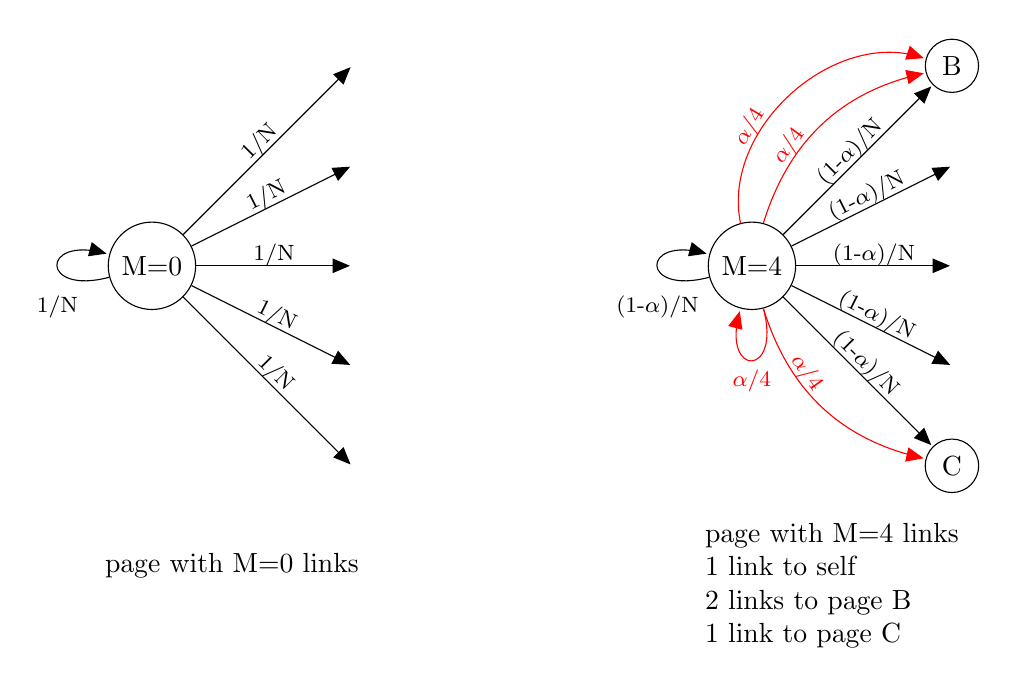
\begin{tikzpicture}[x=1in,y=1in]
\begin{scope}[>=triangle 45,shorten >=0.01in,->]

    \node[shape=circle,draw] (p0) at (0,1) {M=0};

    \draw (p0) edge[anchor=center,loop left]
	           node[pos=0.5,below=0.10in]{\SMALL 1/N} ();
    \foreach \n in {0,0.5,...,2}
	\draw (p0) to node[pos=0.5,sloped,above=-0.05in]{\SMALL 1/N} (1,\n);

    \node at (0.4,-0.5) {
        \begin{tabular}{l}
	page with M=0 links
	\end{tabular}
    };
\end{scope}

\begin{scope}[>=triangle 45,shorten >=0.01in,->,xshift=3in]

    \node[shape=circle,draw] (p4) at (0,1) {M=4};
    \draw (p4) edge[anchor=center,loop left]
	           node[pos=0.5,below=0.10in]{\SMALL (1-$\alpha$)/N} ();
    \foreach \n in {0.5,1.0,...,1.5}
	\draw (p4) to node[pos=0.5,sloped,above=-0.05in]
	           {\SMALL (1-$\alpha$)/N} (1,\n);
    \draw[red] (p4) edge[anchor=center,loop below]
	           node[pos=0.5,below]{\SMALL $\alpha$/4} ();

    \node[shape=circle,draw] (c) at (1,0) {C};
    \draw (p4) to node[pos=0.5,sloped,above=-0.05in]
	           {\SMALL (1-$\alpha$)/N} (c);
    \draw[red] (p4) to[bend right] node[pos=0.33,sloped,above=-0.05in]
	       {\SMALL $\alpha$/4} (c);

    \node[shape=circle,draw] (b) at (1,2) {B};
    \draw (p4) to node[pos=0.5,sloped,above=-0.05in]
	           {\SMALL (1-$\alpha$)/N} (b);
    \draw[red] (p4) to[bend left] node[pos=0.33,sloped,above=-0.05in]
	       {\SMALL $\alpha$/4} (b);
    \draw[red] (p4) to[bend left=60] node[pos=0.33,sloped,above=-0.05in]
	       {\SMALL $\alpha$/4} (b);

    \node at (0.4,-0.6) {
        \begin{tabular}{l}
	page with M=4 links \\
	1 link to self \\
	2 links to page B \\
	1 link to page C \\
	\end{tabular}
    };

\end{scope}
\end{tikzpicture}
\end{document}
